
%%% Uncomment for slide version
\documentclass{beamer}
\usepackage{listings}
\usepackage{adjustbox}

\setbeameroption{hide notes} % Only slides

%%% Uncomment for handout version
%\documentclass[handout]{beamer}
%\setbeameroption{show notes on second screen=right} % Both

\setbeamertemplate{note page}{\pagecolor{white}\insertnote}
\setbeamertemplate{footline}{}
\usetheme[progressbar=frametitle]{moloch}% modern fork of the metropolis theme
\setbeamercolor{background canvas}{bg=white}
\setbeamercolor{progress bar}{use=palette primary,fg=red,bg=red}
\setbeamercolor{note page}{bg=white} 
\setbeamertemplate{date}{}





\defbeamertemplate*{title page}{customized}[1][]
{
	\usebeamerfont{title}\inserttitle\par
	\bigskip
	\bigskip
		\bigskip
			\bigskip

	\usebeamerfont{title}\usebeamercolor[fg]{subtitle}\insertsubtitle\par
	\bigskip
	\usebeamerfont{author}\insertauthor\par
	\usebeamerfont{subtitle}\insertinstitute\par
	\usebeamercolor[fg]{titlegraphic}\inserttitlegraphic
}

\addtobeamertemplate{navigation symbols}{}{%
	\usebeamerfont{footline}%
	\usebeamercolor[fg]{footline}%
	\hspace{1em}%
	\insertframenumber/\inserttotalframenumber
}
\setbeamercolor{itemize item}{fg=black}
\setbeamercolor{itemize subitem}{fg=black}
\setbeamercolor{itemize subsubitem}{fg=black}

\newcommand\blfootnote[1]{%
	\begingroup
	\renewcommand\thefootnote{}\footnote{#1}%
	\addtocounter{footnote}{-1}%
	\endgroup
}


%%%%%%%%%%%%%%%%%%
%%%%%%%%%%%%%%%%%%
%%%%%%%%%%%%%%%%%%
%%%%%%%%%%%%%%%%%%
%%%%%%%%%%%%%%%%%%
%%%%%%%%%%%%%%%%%%
%%%%%%%%%%%%%%%%%%


%%% Slide 1

\title{\Huge FRST302: Forest Genetics}
\author{\Large Lecture 1.1: Classical Genetics and its Molecular Mechanisms}
\date{\today}

\begin{document}
	\maketitle

\note{\emph{Remember, everything on the lecture slides and the accompanying notes is potentially examinable!}}
% for the beamer version
%\documentclass{beamer}


%%% Slide 3
	
\begin{frame}
		\frametitle{Outline for Today}
\setbeamertemplate{itemize items}[circle]
\Large{
			\begin{itemize} 
			\item Short history of genetics
			\item Mendel's laws
			\item Chromosomes
		\end{itemize}
	}

\note{
Learning Outcomes
	\emph{		\begin{itemize} 
				\item Basic definitions in genetics
				\item Principles and terms in classical genetics
				\item Molecular mechanisms of classical genetics
				\item Chromosome crossover and its significance
			\end{itemize}
	}
}
\end{frame}

%%% Slide 4
\begin{frame}
\frametitle{History of Genetics}

\Large \textbf{What is genetics?} \par

\bigskip
\pause
\Large \textbf{Genetics is the study of genes}, of variation and heredity across all branches of the tree of life




\end{frame}



%%% Slide 2

\begin{frame}
	
	\Huge \centering \emph{What are the major questions in genetics?}
	\vspace{20pt}
	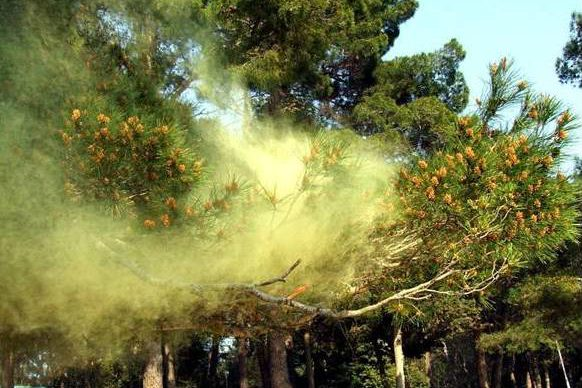
\includegraphics[keepaspectratio, width  =0.8\textwidth]{img/pollenPlume}
	\note{
		The answer to this question totally depends on your perspective. However, I think that it is more than fair to say that the following questions are at the heart of most biological science:
		\begin{itemize} 
			\item Why is there so much variation among individuals?
			\item How is this variation maintained in populations?
			\item Why do offspring tend to resemble their parents? 
			\par
		\end{itemize}
		
		\footnote \url{https://www.asthmacenter.com/wp-content/uploads/Pine-Pollen-Plume-e1495119706845.jpg}
	}
\end{frame}


\begin{frame}
	
	How can we apply a knowledge of genetics?
	
	\vspace{5pt}
	
	\centering
	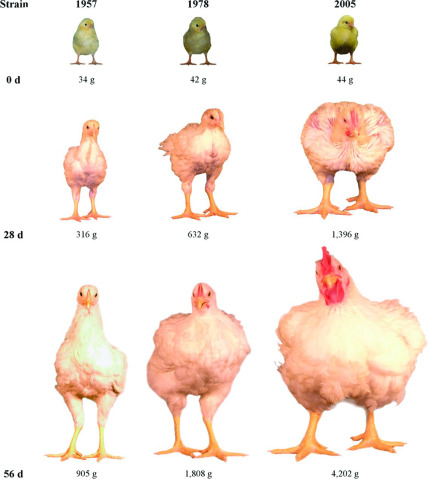
\includegraphics[keepaspectratio, width  =0.6\textwidth]{img/zuidhof_2014} \footnote {Modified from Figure 1 - Zuidhof et al. 2014}
\end{frame}

\begin{frame}
	\frametitle{History of Genetics}
	
\begin{columns}[T]
	\begin{column}{.7\textwidth}
			Humans have probably pondered inheritence for all history:
			\vspace{10pt}
			\begin{itemize}
				\item For much of history, the mechanisms of inheritence were basically unknown
				\item The inheritance of acquired characteristics was widely accepted for much of history (from Hippocrates to Aristotal to Lamarck) \pause
				\item \emph{Early microscopists thought that they had seen small humans inhabiting sperm cells!}
			\end{itemize}
	\end{column}
	\begin{column}{.3\textwidth}
			% Your image included here
% TODO: \usepackage{graphicx} required
\centering
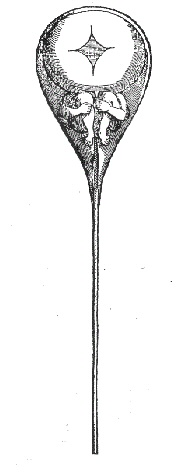
\includegraphics[keepaspectratio, width  = 0.8\textwidth]{img/homunculous}\footnotemark[1]


	\end{column}
\end{columns}
   \note{
	The inheritance of acquired characteristics is often referred to simply as Lamarkism after Jean-Baptiste Lamarck.

	Lamarck was an 19th century evolutionary biologist who formalised a lot of the contemporary thought on how biodiversity originated. The classic example is a giraffe stretching up to reach higher leaves would likely give birth to offspring with longer necks.
	
	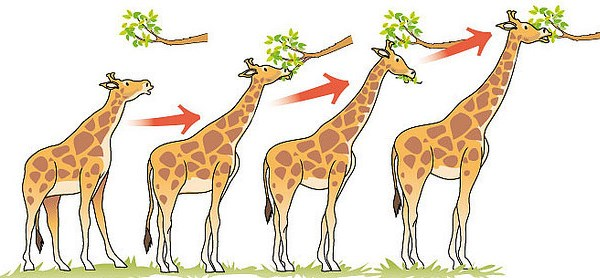
\includegraphics[keepaspectratio, width  = 0.8\textwidth]{img/lamarck}\\
			\url{https://simple.wikipedia.org/wiki/Lamarckism}
}
\end{frame}



\begin{frame}
	\frametitle{History of Genetics}
	
	\begin{columns}[T]
		\begin{column}{.6\textwidth}
			At the time Darwin came around, the dominant theory was \textbf{blending inheritance}
		
			\vspace{5pt}
			\begin{itemize}
				\item The notion that an offspring's traits are simply the average of the parents' traits. 
				\item This is intuitively appealing -  continuously varying traits are often intermediate between their parents 
				\item There is one big problem with blending inheritance!
			\end{itemize}
		\end{column}
		\begin{column}{.3\textwidth}
				\centering
			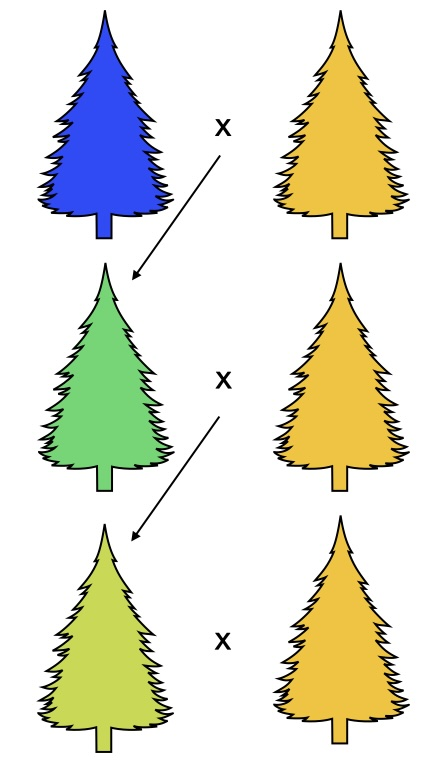
\includegraphics[keepaspectratio, width  = 0.4\textwidth]{img/blending}
		\end{column}
	\end{columns}
	

\end{frame}
	
\begin{frame}
		\frametitle{The Problem with Blending}
		
				\Huge \centering \emph{What's the big problem with blending inheritance?}
		   \note{The halving of variation each generation due to blending inheritance was first pointed out by Fleeming Jenkin - the inventor of the cable car}
\end{frame}



\begin{frame}

	\frametitle{Trait Variation}

	Blending inheritence only really makes sense when you are thinking about continuously varying traits
	\vspace{5pt}

But different modes of variation are common:\pause
\begin{itemize}
	\item Continuous  - traits measured on a numerical scale (e.g. height, diameter, chlorophyll fluorescence) \pause
	\item Discrete - traits that exhibit categorical differences (e.g. different leaf forms, distinct flower colour) \pause
	\item Ordinal - discrete traits with some informative order (e.g. high, medium and low shade tolerance)
	
\end{itemize}

\end{frame}



\begin{frame}
	
	\frametitle{Particulate Inheritance}
	
	\begin{columns}[T]
		
		\begin{column}{0.6\textwidth}
			
			Through careful experimentation analysing discrete traits in peas, Franciscan Friar Gregor Mendel found evidence supporting a model of paticulate inheritence
			
			\vspace{10pt}
			
			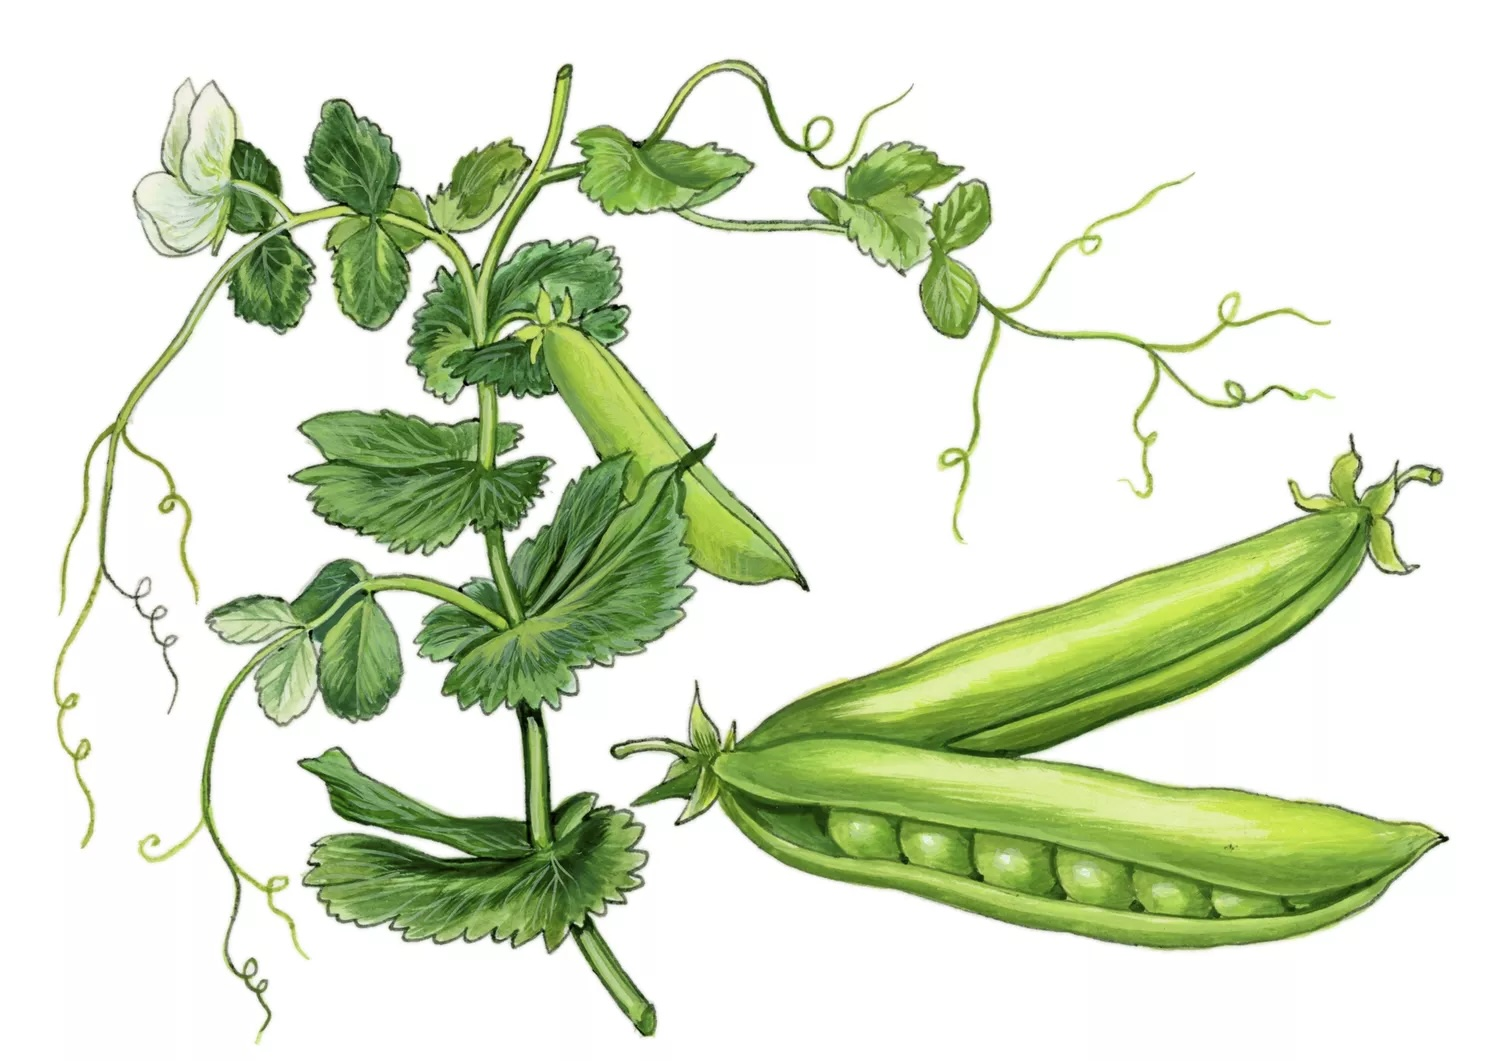
\includegraphics[keepaspectratio, width  =0.8\textwidth]{img/peas}
			
		\end{column}
		\begin{column}{.4\textwidth}
			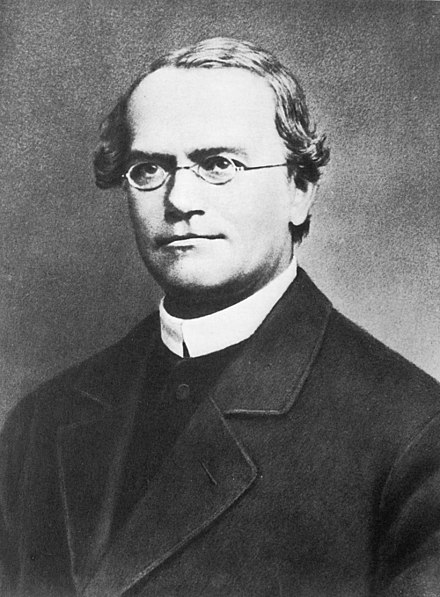
\includegraphics[keepaspectratio, width  =\textwidth]{img/mendel}
			\centering
			Mmmmm...\\
			Peas Peas Peas Peas Peas
		\end{column}
		
		\note{Pea pic from: \url{https://www.thoughtco.com/domestication-history-of-peas-169376}}
		
		
	\end{columns}
\end{frame}




\begin{frame}
	\frametitle{Mendel's Crosses}
	\centering
	Mendel examined variation and inheritence of several discrete characteristics of pea plants
	\vspace{10pt}

			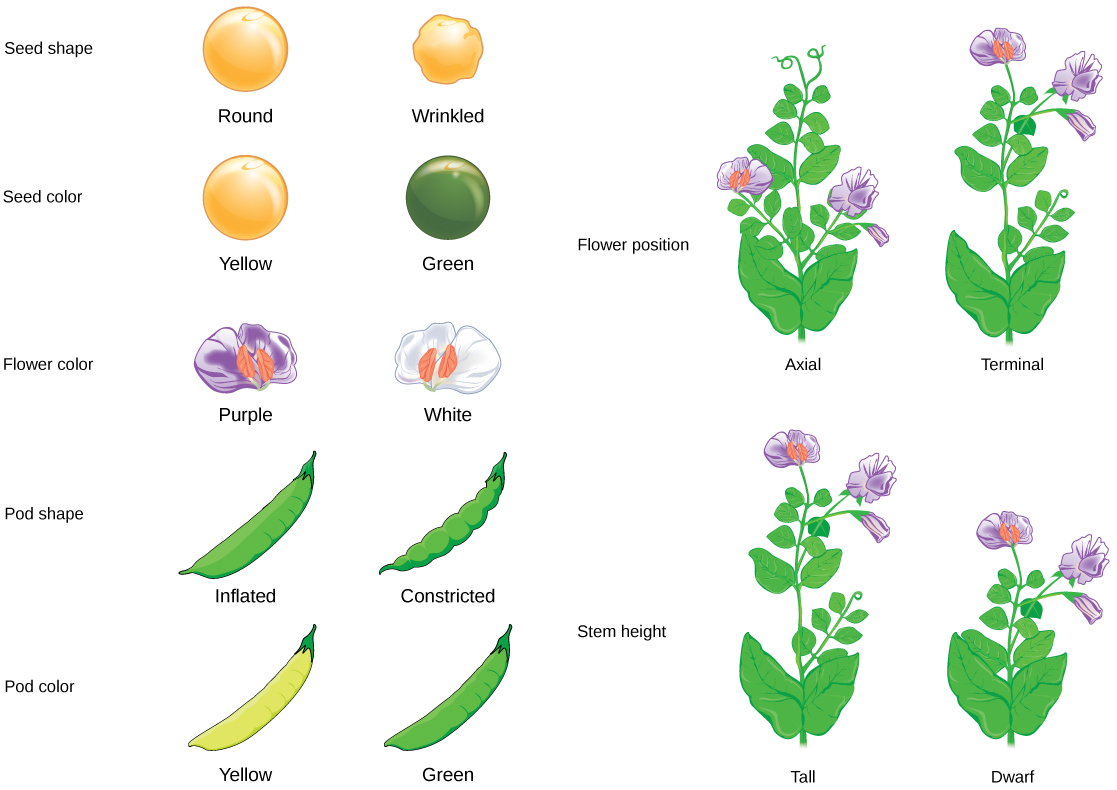
\includegraphics[keepaspectratio, width  =0.8\textwidth]{img/mendelCross_2}
\note{Figure from: \url{https://opentextbc.ca/biology/wp-content/uploads/sites/96/2015/02/Figure_08_01_03.jpg}}
\end{frame}


\begin{frame}
	
	\frametitle{Mendel's Crosses}

	
\begin{columns}
	\begin{column}{0.5\textwidth}
			Garden peas are capable of self-fertilzation, so Mendel was abe to generate "true" lines of peas that exhibit a particular trait/phenotype
		\begin{itemize}
	\item	Crossing lines produces an F1 generation \note{F1 stands for first filial generation. Subsequent crosses of individuals from the F1 generation will produce an F2, crossing individuals from the F2 generation will produce an F3 and so on...}	
	\item 	The patterns of variation among the F2 generations led Mendel to develop his notions of particulate inheritence
		\end{itemize}
		


	\end{column}
	\begin{column}{0.6\textwidth}  
\begin{center}
			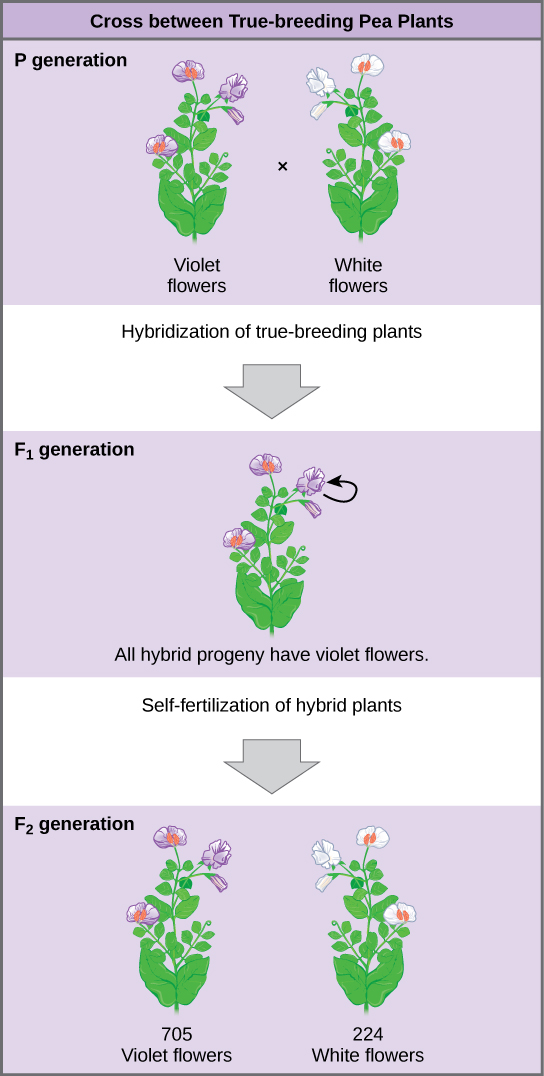
\includegraphics[keepaspectratio, width  =0.6\textwidth]{img/mendelCross_1}
\end{center}
\end{column}
\end{columns}
\end{frame}



\begin{frame}
	
	\frametitle{Particulate Inheritance}
	
	\begin{columns}[T]
		
		\begin{column}{0.6\textwidth}
			
			\begin{itemize}
				\item Proposed in 1865 and 1866
				\item 6-7 years after Darwin’s Theory of Evolution
				\item Represents the foundation of modern genetics
				\vspace{20pt}
				\item ASD
			\end{itemize}
			
			
		\end{column}
		\begin{column}{.4\textwidth}
			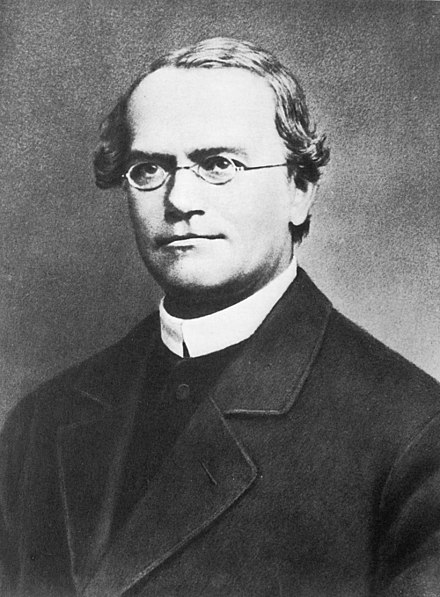
\includegraphics[keepaspectratio, width  =\textwidth]{img/mendel}
			\centering
			More peas please
		\end{column}
		
		\note{Pea pic from: \url{https://www.thoughtco.com/domestication-history-of-peas-169376}}
		
		
	\end{columns}
	\note{
		A letter from Darwin to Alfred Russel Wallace - 6th Februrary 1866
		
		``My dear Wallace,
		
		After I had despatched my last note, the simple explanation which you give had occurred to me, and seems satisfactory.
		
		I do not think you understand what I mean by the non-blending of certain varieties. It does not refer to fertility; an instance will explain; I crossed the Painted Lady and Purple sweet-peas, which are very differently coloured vars, and got, even out of the same pod, both varieties perfect but none intermediate. Something of this kind I shd. think must occur at first with your butterflies got the 3 forms of Lythrum; tho’ these cases are in appearance so wonderful, I do not know that they are really more so than every female in the world producing distinct male got female offspring.
		
		I am heartily glad that you mean to go on preparing your journal.6
		
		Believe me yours,  very sincerely,
		
		Ch. Darwin"}
\end{frame}






\begin{frame}
	\frametitle{Reconciling the Mendelians and the Biometricians}

				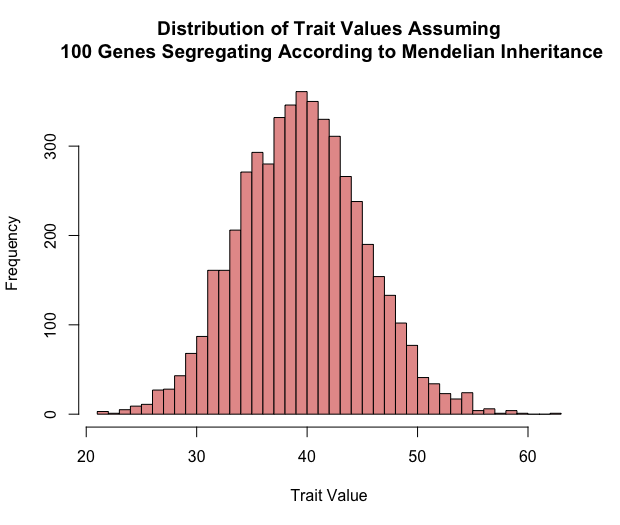
\includegraphics[keepaspectratio, width  =\textwidth]{img/100Genes}
\end{frame}




\begin{frame}[fragile]
	\frametitle{Particulate Inheritance}
	
	\textbf{Below is the R code to make the figures on the infinitesimal model - feel free to play around with it}
	\begin{adjustbox}{max width=\textwidth}
		
	\begin{lstlisting}[language=R]

# Demonstrate the distribution of trait values for a quantitative trait
# Under Mendelian segregation for an arbitrary number of genes
# Assumes random mating, constant effect sizes, constant allele frequencies
	
nGenes = 100
alleleFrequency = 0.2
popSize = 5000
effectSize = 1
			
hist( 
	replicate(popSize,
		sum(  1 * rbinom(nGenes, 2, alleleFrequency) ) ),
	col = "#e69b99",
	xlab=  "Trait Value",
	main= paste("Distribution of Trait Values Assuming\n",nGenes, 
		"Genes Segregating According to Mendelian Inheritance"),
	breaks = 40)
		\end{lstlisting}
\end{adjustbox}
\end{frame}



\end{document}

The Mendelian Biometrician debate was rather fierce. ``Mr. Bateson devotes many words to these questions, but one cannot help feeling that his speculations would have had more value had he kept his emotions under better control; the style and method of the religious revivalist are ill-suited to scientific controversy. It is difficult to speak with patience either of the turgid and bombastic preface to 'Mendel’s Principles,' with its reference to Scribes and Pharisees, and its Carlylean inversions of sentence, or of the grossly and gratuitously offensive reply to Professor Weldon and the almost equally offensive adulation of Mr. Galton and Professor Pearson  Yule 1990}



